\documentclass[11pt]{article}

\usepackage[utf8]{inputenc}
\usepackage[margin=0.82in]{geometry}
\usepackage{amsmath, amssymb, amsfonts}
\usepackage[dvipsnames]{xcolor}
\usepackage{hyperref}
\usepackage{titlesec}
\usepackage{enumitem}
\usepackage{parskip}
\usepackage{array}
\usepackage{longtable}
\usepackage{booktabs}
\usepackage{tabularx}
\usepackage{ragged2e}
\usepackage{forest}
\usepackage{float}
\usepackage{graphicx}
\usepackage{tikz}
\usetikzlibrary{positioning, arrows.meta}

\hypersetup{
    colorlinks=true,
    linkcolor=black,
    urlcolor=blue,
    citecolor=black
}

% --------------------
% Title formatting
% --------------------
\titleformat{\section}
    {\LARGE\bfseries\color{black}}
    {}
    {0pt}
    {}

\titleformat{\subsection}
    {\large\bfseries\color{red}}
    {}
    {0pt}
    {}

\titleformat{\subsubsection}
    {\normalsize\bfseries\color{red}}
    {}
    {0pt}
    {}

\setlength{\parindent}{0pt}
\setlength{\parskip}{6pt}
\setlist[itemize]{leftmargin=1.4em, itemsep=3pt, topsep=3pt}
\setlist[enumerate]{leftmargin=1.6em, itemsep=3pt, topsep=3pt}
\renewcommand{\arraystretch}{1.18}

\newcolumntype{Y}{>{\RaggedRight\arraybackslash}X}
\newcolumntype{P}[1]{>{\RaggedRight\arraybackslash}p{#1}}

\title{CSC111 Project 2 Final Report:\\[4pt] Gomoku AI with Game Tree Search and Board Graph Heuristics}
\author{Kai Zang, Shiyuan Lyu, Seoyun Ju, Emily Ye}
\date{\today}

\begin{document}
\maketitle

\section*{Introduction}

\subsection*{Background and Overview}

Gomoku (Five-in-a-Row) is a two-player board game played on a square grid.\cite{gomoku_ref} Players alternate placing stones, and the goal is to create five consecutive stones horizontally, vertically, or diagonally.\cite{gomoku_ref} Although the rules are simple, the game has substantial strategic depth because a single move may simultaneously create an attacking opportunity, block an opponent threat, strengthen local pressure, and influence several future continuations.

This makes Gomoku a strong setting for computational problem solving. A good move is not determined only by the current visual appearance of the board. Instead, a strong player must reason about future consequences, urgent tactical threats, local board structure, and opponent responses. Because of this, Gomoku is a natural domain for combining multiple CSC111 ideas in one project.\cite{proposal}

In our program, future possibilities are represented using an explicit \texttt{GameTree}, where each node stores a game state and each edge corresponds to a move. At the same time, local spatial relationships on the board are represented using a \texttt{BoardGraph}, where each position is connected to nearby positions. These two structures play different but complementary roles: the tree supports adversarial search over future move sequences, while the graph supports local neighborhood analysis and better move ordering.\cite{alpha_beta_ref}

\subsection*{Motivation}

A major motivation for this project came from CSC111 topics on trees, graphs, and game-state reasoning. We wanted to design a project in which trees and graphs were both genuinely useful, rather than added only to satisfy a requirement.

We chose Gomoku because it is visually intuitive and easy for a user to test interactively, but it is still challenging enough to require interesting computation. Compared with smaller classroom examples, Gomoku has a much larger branching factor. On a \(10 \times 10\) board, there can be many legal moves at each turn, so naive search becomes infeasible very quickly. This naturally creates a need for pruning, candidate filtering, tactical checks, heuristic evaluation, and structured state representation.

We were also interested in building an AI system that is explainable. AI is developing very quickly today, and we want to use this project to better understand some of the underlying logic behind AI systems, rather than treat AI as a black box.

Our Gomoku AI will not be a modern machine learning model, but it still includes fundamental AI ideas: state representation, search, heuristic evaluation, pruning, and decision-making under many possible choices. By implementing these components ourselves, we can better understand how an AI agent ``thinks'' in a structured and computational way. Our project is not based on hidden training or machine learning. Instead, every move comes from explicit computation: representing the board, generating possible futures, evaluating positions, pruning unnecessary branches, and selecting the best move. This makes the AI easier to justify and better aligned with the themes of the course.\cite{handout}

\subsection*{Project Goal}

\textbf{How can we design a Gomoku AI that selects strong moves by combining game tree search (minimax with alpha-beta pruning) and graph-based local board heuristics, while remaining efficient enough for real-time human-vs-AI play in a Pygame interface?}

Our goal was therefore to build a playable Gomoku AI that:
\begin{enumerate}
    \item uses trees and graphs in meaningful computational roles,
    \item makes strategically reasonable decisions through explicit search and heuristics, and
    \item remains responsive enough to support interactive gameplay.
\end{enumerate}

\section*{Datasets}

\subsection*{Program Inputs and Generated Data}

Unlike projects that depend on external CSV files or downloaded real-world datasets, our project primarily uses \textbf{dynamically generated game-state data}. The main ``data'' in our system is produced during gameplay and during hypothetical search.

More specifically, our program creates and uses:
\begin{itemize}
    \item the current board state,
    \item hypothetical future board states generated by search,
    \item candidate move sets generated from occupied board positions,
    \item adjacency relationships between board positions generated from board size,
    \item evaluation scores computed from board patterns and local structure.
\end{itemize}

Because all of this data is produced internally by the program, no external dataset download is required to run the project.

\subsection*{What Counts as Data in This Project?}

Although we do not use a traditional dataset, our project still has rich structured data. The board itself is a structured state representation, candidate moves are derived data, future states form generated search data, and the board graph is a spatial dataset built from the grid.

\begin{table}[H]
\centering
\small
\begin{tabularx}{\textwidth}{|P{3.0cm}|P{2.8cm}|Y|}
\hline
\textbf{Data Category} & \textbf{Source} & \textbf{Role in the Program} \\
\hline
Current board state & Generated during play & Stores the real position seen by the human and AI \\
\hline
Future board states & Generated by search & Represents hypothetical outcomes inside the game tree \\
\hline
Candidate moves & Generated from current board & Reduces branching factor by focusing on relevant empty cells \\
\hline
Board adjacency graph & Generated from board size & Supports local neighborhood analysis and graph-based bonuses \\
\hline
Heuristic scores & Computed from patterns & Estimates how favorable a state is for the AI \\
\hline
\end{tabularx}
\caption{Main forms of data used in our project.}
\end{table}

\subsection*{Testing Data}

During development, we also used hand-constructed board states for debugging and doctests. These included:
\begin{itemize}
    \item immediate winning positions,
    \item forced blocking positions,
    \item open-ended runs,
    \item terminal states,
    \item early-game and mid-game boards.
\end{itemize}

These examples helped verify correctness, but they are embedded directly in the code rather than stored as a separate external dataset.

\section*{Computational Overview}

\subsection*{High-Level Program Structure}

Our project is divided into four Python modules, each with a distinct responsibility.

\begin{table}[H]
\centering
\small
\begin{tabularx}{\textwidth}{|P{2.5cm}|P{2.3cm}|Y|}
\hline
\textbf{File} & \textbf{Main Role} & \textbf{Key Responsibilities} \\
\hline
\texttt{main.py} & Entry point & Starts the program by creating a \texttt{GomokuUI} object and running the game loop \\
\hline
\texttt{gomoku\_ui.py} & User interface & Draws the board and stones, handles mouse and keyboard input, displays status text, and coordinates turns between the human and the AI \\
\hline
\texttt{game\_class.py} & Core data model & Defines \texttt{Move}, \texttt{GomokuState}, \texttt{GameTree}, \texttt{Vertex}, and \texttt{BoardGraph}; handles board logic, winner detection, candidate generation, and adjacency representation \\
\hline
\texttt{data\_computa-
-tion.py} & AI computation & Implements heuristic evaluation, tactical checks, move ordering, tree expansion, alpha-beta pruning, caching, and best-move selection \\
\hline
\end{tabularx}
\caption{Overall structure of the Gomoku project.}
\end{table}

This separation improves clarity and makes the project easier to explain. The interface, game representation, and AI logic are not mixed together. The UI is responsible for displaying the game and handling user input, while all computational reasoning remains in the data and AI modules.

\subsection*{Core Data Types}

The most important custom data types in our program are shown below.

\begin{table}[H]
\centering
\small
\begin{tabularx}{\textwidth}{|P{3.0cm}|P{2.1cm}|Y|}
\hline
\textbf{Data Type} & \textbf{Category} & \textbf{Purpose in the Program} \\
\hline
\texttt{Move} & Immutable data object & Stores a row, column, and player symbol for one move \\
\hline
\texttt{GomokuState} & State representation & Stores the board, next player, and last move; supports move validation, copying, winner detection, terminal checks, and candidate generation \\
\hline
\texttt{GameTree} & Tree & Represents future move sequences for adversarial search \\
\hline
\texttt{Vertex} & Graph helper & Represents one board position and its neighboring positions \\
\hline
\texttt{BoardGraph} & Graph & Stores adjacency between nearby board positions for local analysis \\
\hline
\texttt{SearchContext} & Search helper & Stores the board graph, AI identity, and the transposition table used during search \\
\hline
\end{tabularx}
\caption{Main custom data structures used in the project.}
\end{table}

\subsection*{A Beginner-Friendly Alpha-Beta Pruning Tree}

Before explaining our exact Gomoku AI, it is useful to first look at a much smaller minimax tree. This example is intentionally simple. Its purpose is not to model a full Gomoku game, but to make the logic of alpha-beta pruning completely transparent.

\[
\text{Layer 0: Root MAX}
\rightarrow
\text{Layer 1: MIN nodes}
\rightarrow
\text{Layer 2: leaf values}
\]

\begin{center}
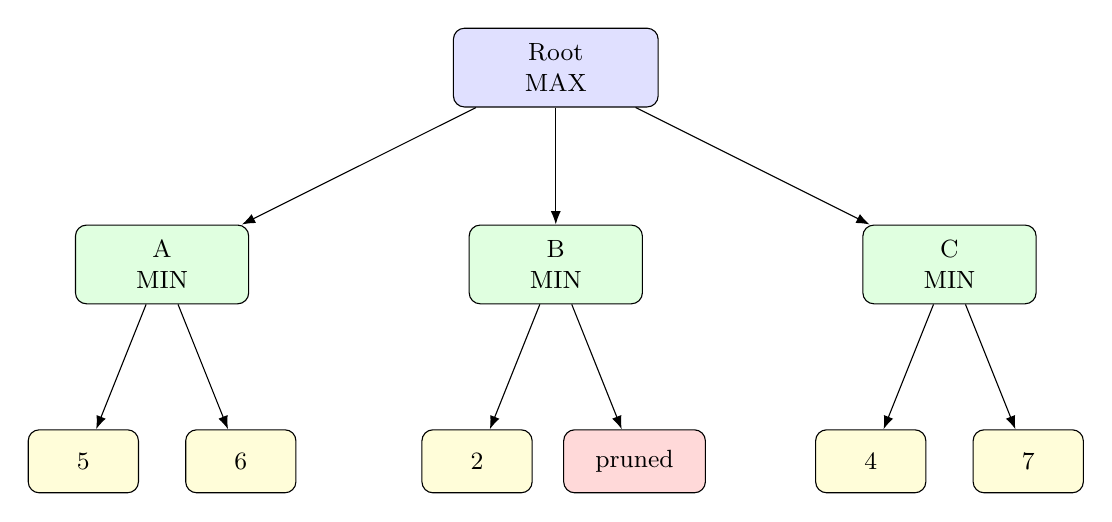
\begin{tikzpicture}[
    >=Latex,
    root/.style={rectangle, rounded corners, draw, fill=blue!12,
        minimum width=26mm, minimum height=10mm, align=center, font=\small},
    minnode/.style={rectangle, rounded corners, draw, fill=green!12,
        minimum width=22mm, minimum height=10mm, align=center, font=\small},
    leaf/.style={rectangle, rounded corners, draw, fill=yellow!15,
        minimum width=14mm, minimum height=8mm, align=center, font=\small},
    pruned/.style={rectangle, rounded corners, draw, fill=red!15,
        minimum width=18mm, minimum height=8mm, align=center, font=\small}
]

\node[root] (root) at (0,0) {Root\\MAX};

\node[minnode] (A) at (-5,-2.5) {A\\MIN};
\node[minnode] (B) at (0,-2.5) {B\\MIN};
\node[minnode] (C) at (5,-2.5) {C\\MIN};

\draw[->] (root) -- (A);
\draw[->] (root) -- (B);
\draw[->] (root) -- (C);

\node[leaf] (A1) at (-6,-5) {5};
\node[leaf] (A2) at (-4,-5) {6};
\draw[->] (A) -- (A1);
\draw[->] (A) -- (A2);

\node[leaf] (B1) at (-1,-5) {2};
\node[pruned] (B2) at (1,-5) {pruned};
\draw[->] (B) -- (B1);
\draw[->] (B) -- (B2);

\node[leaf] (C1) at (4,-5) {4};
\node[leaf] (C2) at (6,-5) {7};
\draw[->] (C) -- (C1);
\draw[->] (C) -- (C2);

\end{tikzpicture}
\end{center}

\noindent
\textbf{What each layer means.}

\begin{center}
\begin{tabularx}{0.96\textwidth}{>{\raggedright\arraybackslash}p{0.16\textwidth} >{\raggedright\arraybackslash}p{0.22\textwidth} X}
\toprule
\textbf{Layer} & \textbf{Node type} & \textbf{Meaning} \\
\midrule
Layer 0 & MAX & The decision-maker wants the largest achievable final value. \\
Layer 1 & MIN & The opponent is assumed to respond optimally, so each node chooses the smallest child value. \\
Layer 2 & Leaf values & These are the already-known outcomes returned to the parent nodes. \\
\bottomrule
\end{tabularx}
\end{center}

\noindent
\textbf{Step-by-step reading of the tree.}

The root is a \textbf{MAX} node, so its job is to choose the branch with the largest final value. Its three children, A, B, and C, are all \textbf{MIN} nodes, which means each of them will return the smallest value among its children.

Node A is evaluated first. Since A is a MIN node and its two leaves are 5 and 6, we obtain
\[
A = \min(5, 6) = 5.
\]
So after finishing A, the root already knows that it can guarantee a value of at least 5. In the language of alpha-beta pruning, the root now has a current \textbf{alpha} value of 5.

Next, we begin exploring node B. The first explored child of B already gives value 2. Because B is a MIN node, its final value can only stay at 2 or become even smaller after exploring more children. In other words, B can never produce a value greater than 2.

At this point, the root already has a branch worth 5 from node A. Since node B can no longer exceed 2, B can never become the root's best choice. Therefore, the second child of B cannot possibly affect the root's final decision, so that branch is safely \textbf{pruned}.

\begin{center}
\begin{tabularx}{0.96\textwidth}{>{\raggedright\arraybackslash}p{0.12\textwidth} >{\raggedright\arraybackslash}p{0.22\textwidth} X}
\toprule
\textbf{Node} & \textbf{Computation} & \textbf{Interpretation} \\
\midrule
A & $\min(5,6)=5$ & A returns 5, so the root now knows it can guarantee at least 5. \\
B & first child $=2$ & Since B is MIN, B can only stay at 2 or decrease, so it cannot beat the root's current best value 5. \\
C & explored only if needed & C is another candidate branch that the root may compare against its current best value. \\
\bottomrule
\end{tabularx}
\end{center}

\noindent
\textbf{Why the pruning is valid.}

The key point is that alpha-beta pruning does \emph{not} guess or approximate the answer. Instead, it proves that certain unexplored branches are already irrelevant. Here, once the root has a guaranteed value of 5 and node B is known to be at most 2, the unexplored part of B cannot possibly change which move the root should choose. So pruning saves work without changing the minimax result.

\noindent
\textbf{Takeaway.} Alpha-beta pruning does \emph{not} change the answer returned by minimax; it only avoids searching branches that are already provably unable to affect the final decision.

\subsection*{Our Gomoku AI Tree (Simplified Depth-Limited Illustration)}

Now we connect this idea to our actual Gomoku project.

In our project, each node is \textbf{not just a number}. Each node stores a full \texttt{GomokuState}. The figure below is a simplified conceptual illustration of our depth-limited search. It is designed to show the logical structure of the algorithm clearly, rather than every branch in the full search tree.

\[
\text{Layer 0: current board}
\rightarrow
\text{Layer 1: AI candidate moves}
\rightarrow
\text{Layer 2: opponent replies}
\rightarrow
\text{Layer 3: evaluation scores}
\]

\begin{center}
\resizebox{\textwidth}{!}{
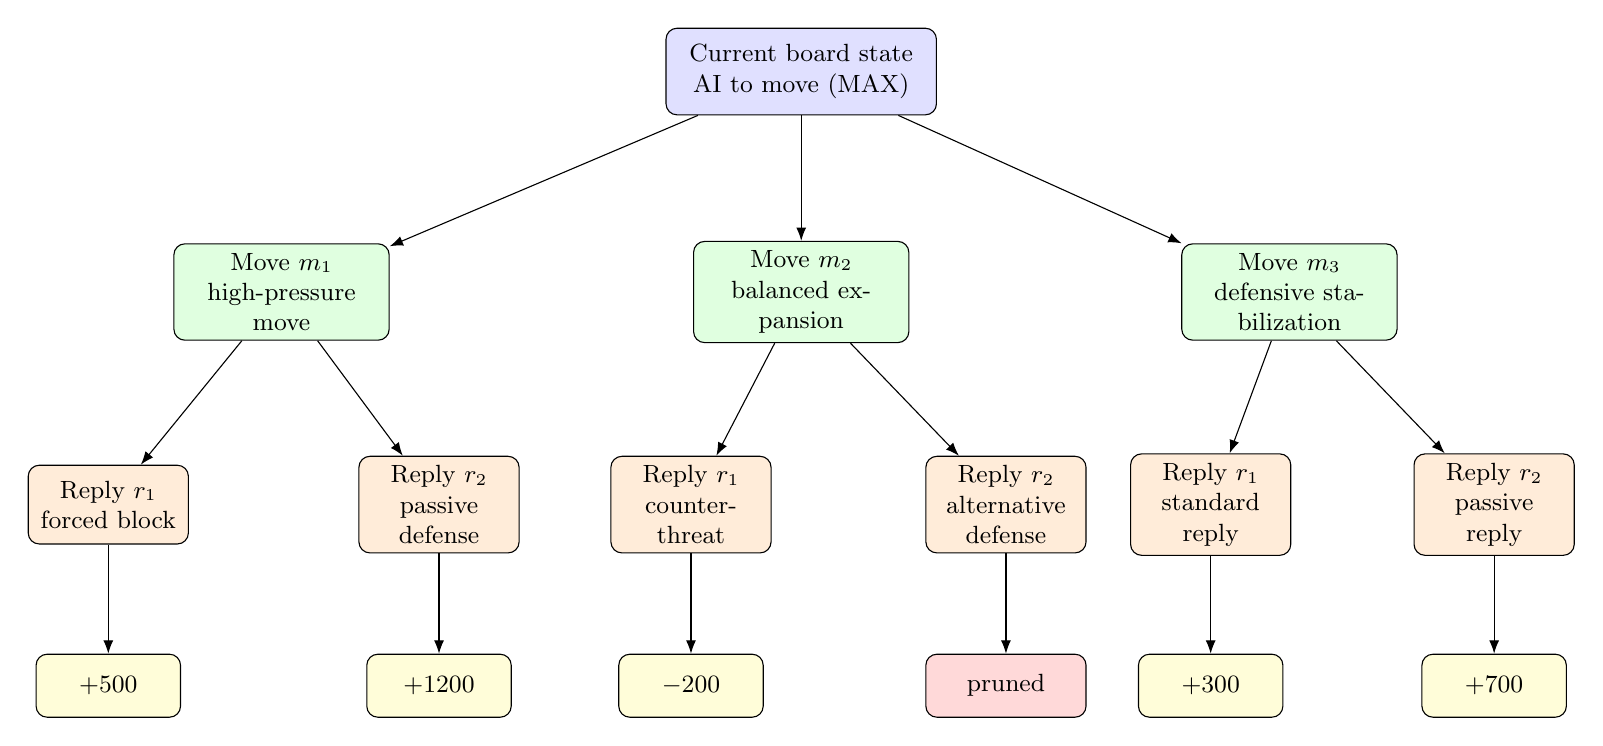
\begin{tikzpicture}[
    >=Latex,
    rootstyle/.style={rectangle, rounded corners, draw, fill=blue!12,
        text width=32mm, minimum height=11mm, align=center, font=\small},
    movestyle/.style={rectangle, rounded corners, draw, fill=green!12,
        text width=25mm, minimum height=10mm, align=center, font=\small},
    replystyle/.style={rectangle, rounded corners, draw, fill=orange!15,
        text width=18mm, minimum height=10mm, align=center, font=\small},
    evalstyle/.style={rectangle, rounded corners, draw, fill=yellow!15,
        text width=16mm, minimum height=8mm, align=center, font=\small},
    prunestyle/.style={rectangle, rounded corners, draw, fill=red!15,
        text width=18mm, minimum height=8mm, align=center, font=\small}
]

\node[rootstyle] (r) at (0,0) {Current board state\\AI to move (MAX)};

\node[movestyle] (m1) at (-6.6,-2.8) {Move $m_1$\\high-pressure\\move};
\node[movestyle] (m2) at (0,-2.8) {Move $m_2$\\balanced ex-\\pansion};
\node[movestyle] (m3) at (6.2,-2.8) {Move $m_3$\\defensive sta-\\bilization};

\draw[->] (r) -- (m1);
\draw[->] (r) -- (m2);
\draw[->] (r) -- (m3);

\node[replystyle] (m1r1) at (-8.8,-5.5) {Reply $r_1$\\forced block};
\node[replystyle] (m1r2) at (-4.6,-5.5) {Reply $r_2$\\passive defense};
\draw[->] (m1) -- (m1r1);
\draw[->] (m1) -- (m1r2);

\node[replystyle] (m2r1) at (-1.4,-5.5) {Reply $r_1$\\counter-\\threat};
\node[replystyle] (m2r2) at (2.6,-5.5) {Reply $r_2$\\alternative\\defense};
\draw[->] (m2) -- (m2r1);
\draw[->] (m2) -- (m2r2);

\node[replystyle] (m3r1) at (5.2,-5.5) {Reply $r_1$\\standard\\reply};
\node[replystyle] (m3r2) at (8.8,-5.5) {Reply $r_2$\\passive\\reply};
\draw[->] (m3) -- (m3r1);
\draw[->] (m3) -- (m3r2);

\node[evalstyle] (m1e1) at (-8.8,-7.8) {$+500$};
\node[evalstyle] (m1e2) at (-4.6,-7.8) {$+1200$};
\draw[->] (m1r1) -- (m1e1);
\draw[->] (m1r2) -- (m1e2);

\node[evalstyle] (m2e1) at (-1.4,-7.8) {$-200$};
\node[prunestyle] (m2e2) at (2.6,-7.8) {pruned};
\draw[->] (m2r1) -- (m2e1);
\draw[->] (m2r2) -- (m2e2);

\node[evalstyle] (m3e1) at (5.2,-7.8) {$+300$};
\node[evalstyle] (m3e2) at (8.8,-7.8) {$+700$};
\draw[->] (m3r1) -- (m3e1);
\draw[->] (m3r2) -- (m3e2);

\end{tikzpicture}
}
\end{center}

\noindent
\textbf{How this Gomoku tree corresponds to our implementation.}

This figure is a simplified conceptual illustration of our depth-limited search. Its purpose is to show the logical structure of our algorithm clearly, rather than to display every branch in the full search space. In our actual implementation, each internal node stores a full \texttt{GomokuState}, and each edge represents one legal move that transforms one state into another.

\begin{center}
\begin{tabularx}{0.96\textwidth}{>{\raggedright\arraybackslash}p{0.16\textwidth} >{\raggedright\arraybackslash}p{0.24\textwidth} X}
\toprule
\textbf{Tree layer} & \textbf{Meaning in the figure} & \textbf{Connection to our code} \\
\midrule
Root node & Current board state & The root stores the current \texttt{GomokuState}, which is the starting position for search. \\
AI move layer & Candidate actions for the AI & These children correspond to candidate moves generated by \texttt{get\_candidate\_moves} and then reordered by our heuristic move-ordering system. \\
Opponent reply layer & Possible responses to each AI move & These nodes represent plausible opponent replies explored by minimax search. \\
Evaluation layer & Scores returned from explored branches & These values come from \texttt{evaluate\_state}, unless the branch is terminated earlier by alpha-beta pruning or a terminal-state check. \\
\bottomrule
\end{tabularx}
\end{center}

\noindent
\textbf{How the search progresses from top to bottom.}

The search begins at the root, which stores the current game position. From this state, the AI generates a reduced set of promising candidate moves rather than expanding every empty square on the board. This is important because Gomoku has a very large branching factor, and unrestricted search would be too expensive.

Each child of the root therefore represents a new board state created after one AI move. From each of these states, the search then considers possible opponent replies. Those replies form the next layer of the tree. At a limited search depth, or when a terminal position is reached, the resulting state is assigned a score. That score is returned upward through minimax, so the AI can compare the long-term consequences of different moves.

\noindent
\textbf{Why the leaves are scores but the internal nodes are states.}

A crucial difference between this tree and the small teaching tree above is that the teaching tree contains abstract numbers at the leaves from the start, while our Gomoku tree stores \emph{game states} at the internal nodes. The score does not exist first and then generate the state; rather, the state is created first, and only later evaluated by our heuristic function. This is why the internal nodes should be understood as full board positions, not as fixed numeric labels.

\begin{center}
\begin{tabularx}{0.96\textwidth}{>{\raggedright\arraybackslash}p{0.26\textwidth} X}
\toprule
\textbf{Concept} & \textbf{Interpretation in our project} \\
\midrule
Internal node & A complete \texttt{GomokuState}, including the board configuration and next player. \\
Edge & One move that transforms a parent state into a child state. \\
Leaf score & A heuristic or terminal evaluation returned after search reaches the stopping condition. \\
Red pruned branch & A subtree skipped because alpha-beta pruning proves it can no longer affect the root's final choice. \\
\bottomrule
\end{tabularx}
\end{center}

\noindent
\textbf{Final interpretation.}

Taken together, this tree shows the full logic of our algorithm: the root stores the current state, the next layer stores candidate AI moves, the following layer stores opponent responses, and the final values represent the outcome of evaluating those future states. The AI then chooses the root move with the best returned score, which corresponds to the strongest move under the search model.

\subsection*{Why Our AI Uses Both a Tree and a Graph}

Our project uses two different data structures for two different purposes.

\textbf{GameTree}
\begin{itemize}
    \item stores possible future board states,
    \item represents ``if we move here, then the opponent may reply here,''
    \item supports minimax and alpha-beta pruning.
\end{itemize}

\textbf{BoardGraph}
\begin{itemize}
    \item stores local adjacency relationships between board positions,
    \item helps reward moves close to friendly stones or strategically active areas,
    \item improves move ordering and local evaluation.
\end{itemize}

So the graph helps the AI understand \textbf{local structure}, while the tree helps the AI reason about \textbf{future consequences}. This division is important because a Gomoku AI needs both perspectives. It must care about immediate local pressure, but it must also care about how the position may develop after several alternating turns.

\subsection*{How the Graph Works}

The graph serves a different purpose from the tree. Our class \texttt{BoardGraph} models the board as an undirected graph:
\begin{itemize}
    \item each board position is a vertex,
    \item edges connect neighboring positions,
    \item diagonal neighbors are included, so each interior position can have up to eight neighbors.
\end{itemize}

The graph is built once when the board is initialized. It is then used for local spatial analysis. In particular, the method \texttt{positions\_within\_distance} performs a BFS-style search and returns nearby positions around a chosen move.

This supports the function \texttt{graph\_local\_bonus}, which gives a small bonus to moves near friendly stones and a smaller bonus to moves near enemy stones. The intuition is that strong Gomoku moves usually appear near active parts of the board rather than in isolated empty corners. The graph therefore helps the AI focus on strategically relevant areas and improves move ordering.

\subsection*{Heuristic Evaluation}

For non-terminal states, our AI uses a custom evaluation function \texttt{evaluate\_state}. This function returns an integer score from the AI's perspective:
\begin{itemize}
    \item positive scores favor the AI,
    \item negative scores favor the opponent.
\end{itemize}

The evaluation combines several ideas.

\begin{table}[H]
\centering
\small
\begin{tabularx}{\textwidth}{|P{4.0cm}|Y|}
\hline
\textbf{Evaluation Component} & \textbf{Purpose} \\
\hline
Length-5 window scoring & Scores critical Gomoku patterns such as four-in-a-row with one empty cell \\
\hline
Open-ended run scoring & Distinguishes stronger open runs from weaker blocked runs \\
\hline
Center-control bonus & Slightly rewards stones closer to the center of the board \\
\hline
Graph-based local bonus & Rewards moves near active stones and local tactical regions \\
\hline
Immediate tactical bonus & Strongly rewards moves that create an immediate win \\
\hline
\end{tabularx}
\caption{Main components of the heuristic evaluation function.}
\end{table}

The board is analyzed across rows, columns, and both diagonal directions. This allows the AI to recognize both offensive opportunities and defensive threats. A good evaluation function in Gomoku must do more than count stones. It must distinguish between weak structures and dangerous structures. For example, an open-ended run of three stones is often much more valuable than a blocked run of three, because it creates more future winning opportunities. Our scoring system was designed to reflect this difference.

\subsection*{Efficiency Improvements}

A full search on a \(10 \times 10\) board is too expensive, so our AI includes several efficiency improvements.

\begin{enumerate}
    \item \textbf{Candidate move reduction:} instead of considering every empty square, the AI mainly considers empty positions near occupied cells.
    \item \textbf{Immediate tactical checks:} before deeper search, the AI checks whether an immediate winning move exists.
    \item \textbf{Move ordering:} more promising branches are searched earlier.
    \item \textbf{Safe root filtering:} moves that immediately allow an opponent win are avoided when possible.
    \item \textbf{Transposition table caching:} repeated states can reuse previously computed scores.
\end{enumerate}

\begin{table}[H]
\centering
\small
\begin{tabularx}{\textwidth}{|P{4.0cm}|Y|}
\hline
\textbf{Optimization} & \textbf{Why It Helps} \\
\hline
Candidate moves near occupied cells & Greatly reduces branching factor \\
\hline
Ordered move search & Helps strong branches appear earlier, increasing pruning \\
\hline
Immediate-win detection & Resolves urgent tactical cases without deeper search \\
\hline
Safe root filtering & Prevents obviously losing choices when possible \\
\hline
Transposition table & Avoids recomputing repeated states \\
\hline
\end{tabularx}
\caption{Efficiency improvements in the final AI design.}
\end{table}

These improvements are especially important in an interactive project. Our AI is not trying to solve Gomoku perfectly. Instead, it is trying to make strong and reasonable decisions within a short response time so that the human player can enjoy a smooth game experience.

\subsection*{Overall AI Pipeline}

The full AI decision process can be summarized as follows:

\begin{enumerate}
    \item Represent the current board as a \texttt{GomokuState}.
    \item Generate a reduced set of candidate moves.
    \item Check for an immediate winning move.
    \item Prefer safe root moves when possible.
    \item Expand one layer of \texttt{GameTree} children.
    \item Order moves using heuristics and graph-based local bonuses.
    \item Run minimax with alpha-beta pruning.
    \item Return the best move and play it in the interface.
\end{enumerate}

\texttt{The algorithm can be understood even more simply}:
\begin{enumerate}
    \item start from the current board,
    \item try several promising moves for the AI,
    \item imagine how the opponent may respond,
    \item score the resulting states,
    \item stop exploring branches that are already clearly worse,
    \item choose the move with the best final score.
\end{enumerate}

This pipeline shows that our AI is not based on one isolated idea, but on several coordinated components working together.

\subsection*{Interactive Visualization with Pygame}

We used the \texttt{pygame} library to create a playable graphical interface.\cite{pygame_docs} This is the main external library used in the project.

Our class \texttt{GomokuUI} is responsible for:
\begin{itemize}
    \item drawing the board and grid,\cite{pygame_display}
    \item drawing black and white stones,
    \item highlighting the most recent move,
    \item drawing a winning line after the game ends,
    \item displaying status text,\cite{pygame_font}
    \item handling mouse and keyboard input,
    \item coordinating turns between the human and the AI.
\end{itemize}

We intentionally kept the interface clean and readable. The focus of the project is the computational logic, but the interface still makes the system interactive and easy to test. This interactive component is important for the project because it allows the TA to observe the AI's behavior directly rather than only reading internal scores.

\section*{Instructions for Running the Program}

\subsection*{Required Files}

The submission should include:
\begin{itemize}
    \item \texttt{project\_report.tex}
    \item \texttt{project\_report.pdf}
    \item \texttt{requirements.txt}
    \item \texttt{main.py}
    \item all other Python modules used by the project
\end{itemize}

All Python files should be kept in the same folder.

\subsection*{Required Libraries}

The required external libraries are listed in \texttt{requirements.txt}. The main packages are:
\begin{itemize}
    \item \texttt{python-ta}
    \item \texttt{pygame}
\end{itemize}

Built-in modules such as \texttt{typing}, \texttt{dataclasses}, and \texttt{doctest} do not need separate installation.
Our implementation still relies on these built-in modules for type annotations and structured data modeling.\cite{python_typing,python_dataclasses}

\subsection*{Datasets and Downloads}

No external dataset is required for this project. Our program generates and evaluates game states dynamically during play, so there is no CSV file, zip download, or preprocessing dataset that the TA must obtain separately.

\subsection*{Running the Program}

To run the project:
\begin{enumerate}
    \item Install Python 3.13.5.
    \item Put all submitted Python files in the same folder.
    \item Install the libraries listed in \texttt{requirements.txt}.
    \item Run \texttt{main.py}.
\end{enumerate}

No external dataset download is required.

\subsection*{What the TA Should Expect to See}

When \texttt{main.py} is run, a Pygame window opens showing a Gomoku board. The human player plays as \texttt{X}, and the AI plays as \texttt{O}.

The TA should expect:
\begin{itemize}
    \item \textcolor{red}{It is extremely challenging for the human player to win against the AI in normal gameplay.}
    \item clicking near an empty grid intersection places a human stone,
    \item after the human move, the AI computes and plays automatically,
    \item the bottom panel displays current status text,
    \item the most recent move is highlighted with a small red marker,
    \item when a win occurs, a red line is drawn through one winning sequence,
    \item pressing \texttt{R} restarts the game,
    \item pressing \texttt{Q} quits the program.
\end{itemize}

\subsection*{Interactive Features}

The project includes:
\begin{itemize}
    \item direct human-vs-AI gameplay,
    \item real-time visual updates after each move,
    \item automatic AI responses,
    \item end-of-game detection and winner display,
    \item restart and quit controls.
\end{itemize}

\subsection*{Suggested TA Testing Strategy}

A simple way to test the project is:
\begin{enumerate}
    \item run the program,
    \item place several human stones in a row or near each other,
    \item observe whether the AI responds in locally meaningful positions rather than far away random positions,
    \item continue until a clear threat or winning line appears,
    \item verify that the program ends correctly and that restart/quit controls work.
\end{enumerate}

This interaction should be enough to observe that the AI is not random. Instead, it uses search and heuristics to react to the board state in a structured way.

\section*{Changes from Proposal to Final Submission}

\subsection*{Major Changes}

Our final implementation remained faithful to the main idea from the proposal, but several aspects became more refined during development.

First, our proposal emphasized minimax, alpha-beta pruning, graph-based local analysis, and a Pygame interface. All of these ideas were successfully implemented. However, the final project became more sophisticated than the original plan.

One important improvement was the addition of a \texttt{SearchContext} dataclass containing a transposition table. During implementation, we realized that repeated states could appear during search, so caching became useful for reducing recomputation.

Second, the evaluation function became more detailed than originally planned. In addition to length-5 window scoring, the final version includes open-ended run scoring, center-control bonuses, tactical bonuses for immediate wins, and graph-based local bonuses. These changes improved the AI's behavior and made its decisions more natural.

Third, candidate move reduction turned out to be more important than expected. Restricting the search to nearby positions was essential for keeping the AI responsive in an interactive game. Our earlier idea was more search-heavy, but in practice we needed a better balance between search depth and search quality.

\subsection*{UI Refinement}

We also simplified the UI compared with some earlier ideas. Instead of adding too many debug displays or decorative elements, we chose a cleaner final interface focused on:
\begin{itemize}
    \item board clarity,
    \item move visibility,
    \item win visualization,
    \item stable interaction.
\end{itemize}

This made the final submission easier to test and more polished overall. We concluded that for this project, a clear interface was more valuable than a visually overloaded one.

\subsection*{Conceptual Clarification}

Another important change from the proposal was in how we explained the algorithm. During development, we realized that our original description of minimax and alpha-beta pruning was technically correct but not always easy for a beginner to follow. As a result, we revised the final report to include a small teaching tree and a separate simplified Gomoku search tree.

This helped us communicate the project more clearly. Instead of immediately presenting the full implementation, we now begin with a very small alpha-beta example and then connect that idea to our actual \texttt{GameTree}-based search. This makes the computational overview more readable and better demonstrates the reasoning behind the final design.

\section*{Discussion}

\subsection*{Results and Interpretation}

Overall, we believe our final project successfully achieves its main goal. The completed system demonstrates that trees and graphs can work together meaningfully in one application rather than appearing as separate or artificial requirements. The \texttt{GameTree} allows the AI to reason about future possibilities under adversarial play, while the \texttt{BoardGraph} helps it focus on strategically active local regions. These two structures support different forms of reasoning, and together they create a much more interesting AI than either one alone would produce.

One major strength of the project is that the AI does not rely on only one computational idea. Instead, it combines candidate generation, tactical checking, heuristic evaluation, move ordering, explicit game-tree expansion, alpha-beta pruning, and transposition-table caching. This layered design matters because Gomoku is difficult for a naive search strategy. If the AI tried to explore all legal moves uniformly, the branching factor would grow too quickly and interactive play would become too slow. Our final design solves this by combining multiple smaller strategies rather than depending on one single technique.

A second strength is that the graph is not merely decorative. It genuinely affects computation by identifying nearby active positions and rewarding locally meaningful moves. This improves move ordering and indirectly strengthens pruning because stronger candidate branches are searched earlier. In other words, the graph contributes both strategic value and computational efficiency.

A third strength is the interface. The Pygame window makes the project much easier to understand and evaluate. Instead of only printing scores or board states in the terminal, the user can directly observe the AI's behavior. In gameplay, the AI often responds near existing pressure points, blocks obvious threats, and extends its own developing lines. This visual feedback helps demonstrate that the search and heuristic system is functioning in a meaningful way.

\subsection*{Limitations}

At the same time, our project has several limitations.

First, the search depth is still modest. Even with pruning and candidate reduction, deeper search becomes expensive quickly. As a result, the AI is reasonably strong for a course project and clearly better than random play, but it is not expert-level Gomoku.

Second, the evaluation function is hand-designed. Although the scoring rules are intuitive and useful, the weights were chosen manually rather than learned from data or optimized systematically. This means the AI may still misjudge some positions, especially when several tactical ideas compete at the same time.

Third, we did not perform a large empirical benchmark. Through repeated gameplay, we can observe that the AI behaves sensibly and consistently, but we do not yet have a formal comparison against baseline agents across many trials. Such experiments would make our conclusions stronger.

Fourth, our implementation prioritizes clarity and course-aligned design over maximum raw playing strength. This was an intentional tradeoff. We wanted the data structures and algorithms to be understandable, modular, and explainable. That decision improved the educational quality of the project, but it also means we did not pursue some more advanced Gomoku-specific optimizations.

\subsection*{Future Work}

There are several natural next steps for further exploration.

One direction would be to add multiple AI difficulty levels by adjusting search depth, candidate filtering, or heuristic aggressiveness. Another would be to compare different evaluation functions in a more systematic experimental setting. We could also explore more advanced Gomoku techniques such as threat-space reasoning, pattern databases, or stronger pruning rules.

From a software perspective, the interface could be extended with move history, undo support, difficulty selection, or a displayed score estimate for the current position. From an AI perspective, self-play could be used to tune heuristic weights automatically, or to generate large collections of test positions for evaluation.

\subsection*{Final Reflection}

Overall, our project shows that even without an external dataset, a Python program can still demonstrate substantial computational complexity through carefully designed data structures, algorithms, and interaction. The combination of trees, graphs, heuristics, pruning, caching, and a playable interface allowed us to produce a meaningful and polished final system. Most importantly, the project answers the central question we posed at the beginning: it is possible to design a Gomoku AI that combines game-tree search and graph-based local heuristics in a way that is both strategically reasonable and fast enough for real-time human interaction.



\begin{thebibliography}{99}

\bibitem{handout}
University of Toronto CSC111 Course Team.
\textit{CSC111 Project 2 Phase 2: Final Submission Handout}.
Winter 2026.

\bibitem{proposal}
University of Toronto CSC111 Course Team.
\textit{CSC111 Project 2 Phase 1: Proposal Handout}.
Winter 2026.

\bibitem{pygame_docs}
Pygame Community.
\textit{Pygame Documentation}.
Available at: \url{https://www.pygame.org/docs/}

\bibitem{pygame_display}
Pygame Community.
\textit{pygame.display --- pygame documentation}.
Available at: \url{https://www.pygame.org/docs/ref/display.html}

\bibitem{pygame_font}
Pygame Community.
\textit{pygame.font --- pygame documentation}.
Available at: \url{https://www.pygame.org/docs/ref/font.html}

\bibitem{python_dataclasses}
Python Software Foundation.
\textit{dataclasses --- Data Classes}.
Python Standard Library Documentation.
Available at: \url{https://docs.python.org/3/library/dataclasses.html}

\bibitem{python_typing}
Python Software Foundation.
\textit{typing --- Support for type hints}.
Python Standard Library Documentation.
Available at: \url{https://docs.python.org/3/library/typing.html}

\bibitem{gomoku_ref}
Wikipedia contributors.
\textit{Gomoku}.
Available at: \url{https://en.wikipedia.org/wiki/Gomoku}

\bibitem{alpha_beta_ref}
GeeksforGeeks.
\textit{Alpha-Beta Pruning in Adversarial Search Algorithms}.
Available at: \url{https://www.geeksforgeeks.org/artificial-intelligence/alpha-beta-pruning-in-adversarial-search-algorithms/}

\end{thebibliography}

\end{document}
